\chapter{Introduction}\label{chap:intro}
\section{Background}

Electric motor can be classified into two major categories which are the DC electric motor and AC electric motor. An AC motor is an electric motor driven by alternating current whereas a DC motor is driven by direct current. There are various types of AC motor which includes induction motor, synchronous motor, eddy current motor and etc. The DC electric motor includes permanent magnet brushed motor, permanent magnet brushless motor, switched reluctance motor and etc.

Electric motor is used in many application which includes in machine for driving the pulley and belts, the conveyor belt, in drilling and lathe machine. Apart from the heavy industry, electric motor is used in home appliances for powering the washing machine, fan, blower of air-conditioner and blender machine. Moreover, electric motor is also used in automobile industry as the starter motor for firing up the internal combustion engine of cars and trucks and last but not least, as the drive train for electric vehicle.

The PMBLDC is a synchronous motor. In other words, the frequency of the magnetic field generated at the stator and the rotor is the same. PMBLDC comes in single-phase, 2-phase and 3-phase configuration which the 3-phase configuration is the most popular among the three. There are basically two major components inside a PMBLDC motor which is the stator and the rotor. The stator of a PMBLDC motor is made up of 
a series of laminated steel with wire windings around it. The rotor is build up of permanent magnet that has at least 2 poles.

Unlike brushed motor, PMBLDC does not have brushes for comutation, instead a controller is needed for controlling the rotation of the PMBLDC by sending out AC signal to the PMBLDC. There are two types of AC signal sent to the PMBLDC for controlling the motor which are the Trapezoidal type and the Sinusoidal type which depends on the winding of the stator.

In order for the controller to send out the correct signal, the position of the rotor must be sent to the controller so that a sequence of AC signal can be generated which energized the winding of the stator for rotating the motor. Hall effect sensors is used as the rotor position detection sensor which has an analog signal output. When the magnetic field is detected by the hall effect sensor, the voltage output will be changes from lowest to the highest or vice versa depending on the circuit configuration. Normally there are three hall effect sensor mounted on the stator of PMBLDC motor which are 60\textdegree or 120\textdegree apart depending on the number of poles and the comutation sequence required.

Figure \ref{im:signals} shows the hall effect sensors signal for a 2 pole PMBLDC motor, the back emf, the phase current and the output torque. As shown in the figure, there are 3 hall effect sensors with labels A, B and C respectively, sensor A is leading sensor B by 60\textdegree and sensor B is leading sensor C by 60\textdegree. 

%%The back EMF is generated by each of it's stator winding when the motor is rotating which has an opposite direction to the supply voltage which agrees to Lenz's law stating that "An induced electromotive force always give rise to a current whose magnetic field opposes the original change in magnetic flux". Therefore, from figure 1.1, it can ......

Ideally, the phase current should behave as a digital square wave signal where the current rises and drops immediately. But in real world, the current would take some time to rises from zero to maximum/minimum. Hence, the torque produced would behave as a series of ripple instead of a constant output torque.

\begin{figure}
	\centering
	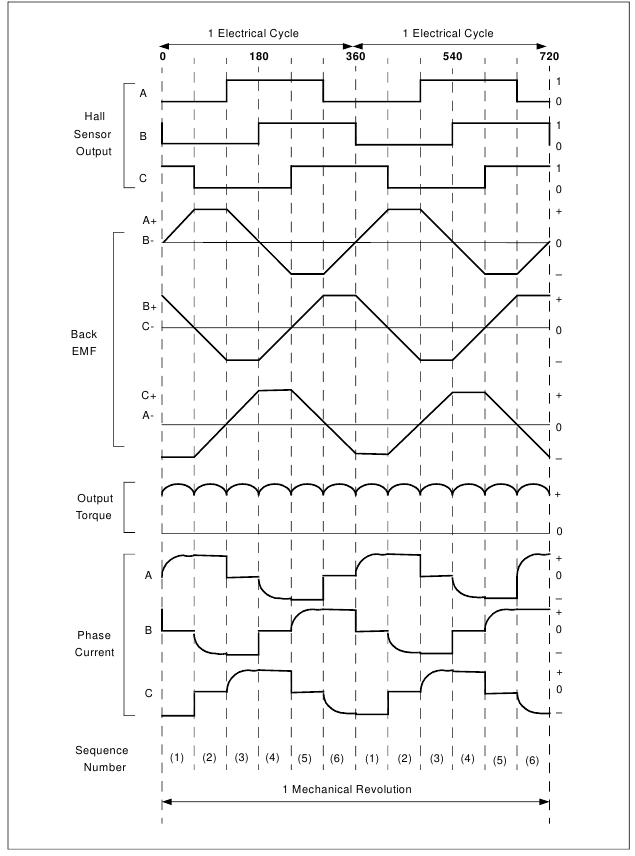
\includegraphics[width=5.5in]{images/signal.jpg}
	\caption{Hall effect sensors signal, back emf, output torque and phase current \citep{an885}}
	\label{im:signals}
\end{figure}

In this project, a PMBLDC hub motor is used as the sole powertrain of a electric vehicle. The electric vehicle will be used for participating the Shell Eco-Marathon which is a competition which teams compete to build a higher mileage vehicle. The competition requires the participating teams to build their own car for the categories they are participating( for example, the urban concept category or the prototype category). For our case, a four-wheel electric vehicle is built for participation in urban concept category. The vehicle will be driven around a race track, which is the Sepang Internation Track, North Track for year 2012 for four laps with 10 seconds of stop between each lap. The energy consumption will be collected and the mileage will be calculated for each attempt and every team will have 3 attempts for mileage improvement.

\section{Problem Statement}
PMBLDC motor is better compare to brushed DC motor because brushless motor increases the efficiency by dropping the friction between the brush and the comutator which happens in brushed DC motor. However, the inefficient PWM in controlling the speed of the motor and the torque ripple cause by the phase current limits the efficiency of a PMBLDC motor.

There are three types of torque produced by a permanent magnet electric motor which are:

\begin{itemize}
	\item cogging torque
	\item reluctance torque
	\item mutual torque
\end{itemize}

The cogging torque is produced by the interaction between the permanent magnet at the rotor and the stator slots. Cogging torque is an undesireable torque generated by the electric motor which dominates at low speed and results in speed ripple. Cogging torque can only be minimize by means of hardware tuning which includes altering the number of poles, teeth at the stator or editing the controller setting which changes the drive current waveform.

The reluctance torque is generated by the difference in position of the rotor and the phase induction at the rotor. The ripple produced by the reluctance torque could be negligible with a good number of poles and slots of the windings at the stator.

The third type of torque produced by PMBLDC motor is the mutual torque which is caused by the non-sinusoidal signal reaching the stator windings or the magnet at the rotor. Since the torque is generated by the current, ripple reduction for mutual torque could be achieved by fine-tuning the current signal.

The torque ripple occurs in PMBLDC is mainly contributed by the different rise and decay time of the phase current as shown in figure \ref{im:signals}. The cogging torque does contribute to torque ripple in low speed but it's negligible at high speed. Torque ripple contributed by reluctance torque could also be ignored since the high number of poles and stator slot minimize the ripple. Mutual torque would be the major contributor to torque ripple due to the direct dependency on the current.

Based on figure \ref{im:comutation} (a), the rate of decay of $i_a$ is faster than the rate of increase of $i_b$. Therefore, at certain point where $i_a$ reaches 0 but $i_b$ still rising, there will be a surge in current at phase C, $i_c$. As the result, there will be a sudden drop in torque output. The same case happens as shown in figure \ref{im:comutation} (c) where $i_a$ drops slower than $i_b$ causing an sudden drop in $i_c$ and sudden increase in torque output. The same circumstances apply for $i_a$-$i_c$ and $i_b$-$i_c$ hence creating a ripple torque output. 

\begin{figure}[htb]
	\centering
	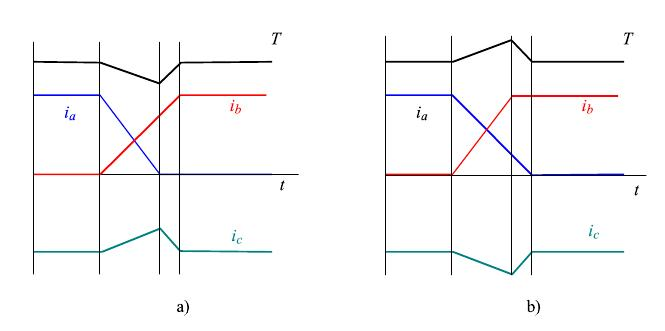
\includegraphics[width=5.5in]{images/phase_current.jpg}
	\caption{The phase current and torque during an alternating comutation event  \citep{7648}}
	\label{im:comutation}
\end{figure}

Apart from torque ripple in PMBLDC that reduce the efficiency of the electric motor and cut down the mileage of the electric vehicle, poor driving strategy will also contributes to poor mileage. The Sepang North Track is a racing track that contains 3 uphill section and 3 uphill section and an approximately 800m long straight for the starting and ending line. This track is especially challenging for electric vehicle because the factor of torque generated by the electric motor, cruise speed when uphill and downhill, rolling resistance and drag factor need to be taken into consideration for minimum energy consumption.

\section{Objectives}

The objectives for this project are:

\begin{enumerate}
	\item To identify the output signal of the controller circuit and the hall effect sensor of the PMBLDC and develop a set of instrument for measuring the mileage of the electric vehicle.
	\item To study the track profile of Sepang North Track and compose a set of strategy to increase the mileage of the electric vehicle.
	\item To suggest methods for improving the efficiency of the electric vehicle through altering the drive current waveform and reducing coefficient of drag.
\end{enumerate}

\section{Scope of Research}

In this project, the proprietary controller and PMBLDC motor signal output port will be identified. After that, by utilizing the signal output of the hall effect sensor and the controller speed output signal port, a set of instrument will be build for measuring the speed, input current and input voltage. The power input will then be calculated based on the voltage and current input.

After the instrumentation for measuring the performance of the electric vehicle is established, methods for improving the overall electric vehicle efficiency will be suggested which includes reducing the frontal area and improving the coefficient of drag of the electric vehicle and hence reducing the drag force. Modification on the phase current signal using indirect method also will be suggested for reducing the torque ripple and hence improving the overall efficiency of the electric vehicle.

Next up, the behaviour of the electric vehicle on the Sepang North Track will be simulated with taking the drag force, rolling resistance and track gradient into consideration. With the frontal area, coefficient of drag, coefficient of rolling resistance and the mass of the vehicle as manipulating variables, a set of strategies could be created for electric vehicle at different mass, tyre pressure at the same track with using the same electric motor as drive train.

\section{Research Approach}

For tapping the signal from the PMBLDC motor's hall effect sensors as well as the analog/digital output from the controller circuit board for the speed signal, multimeter will be used. For building the measurement tools for measuring and logging the input voltage, input current and the speed of the vehicle, Arduino boards will be used in conjunction with the self-made transducing circuit.

For simulating the vehicle's behaviour on track, self-made codes using C++ language will be used for iteration. Data's for each set of simulation and strategies will be saved and the graph will be plot for analysing the effectiveness of the strategy.
